\section{Results and Discussion}
\label{sec:results}

% Every number below comes from results/test_episodes.csv, results/test_summary.csv,
% results/cologne3_per_intersection.csv and the val_log.csv files;
% regenerate with: python paper/make_figures.py and python per_intersection.py

\subsection{Comparison of RL Algorithms}
Table~\ref{tab:main} compares all controllers over the ten test files of each scenario. A2C has the lowest mean waiting time in all three scenarios: 13.5, 10.0 and 25.5\,s, against 32.5, 24.2 and 30.9\,s for fixed-time control. On the single-intersection scenarios, A2C and PPO beat fixed-time in every seed ($p<0.001$, one-sample $t$-test), and A2C beats PPO (Welch's $t$-test, $p=0.030$ and $0.017$). DQN and Double DQN are competitive on ingolstadt1 (10.8 and 11.6\,s, $p<0.001$), but on cologne1 one seed of each gridlocks at $1.3\times$ demand, so their means do not differ significantly from fixed-time ($p=0.95$ and $0.78$) although their medians (18.7 and 19.6\,s) are far lower. Actuated control is worse than fixed-time on cologne1 and ingolstadt1 but better on cologne3, and random control is far worse except on lightly loaded ingolstadt1.

\begin{table}[t]
\caption{Average Total Waiting Time per Vehicle (s)}
\label{tab:main}
\centering
\footnotesize
\setlength{\tabcolsep}{3pt}
\resizebox{\columnwidth}{!}{%
\begin{tabular}{|l|r|r|r|r|r|r|}
\hline
\multirow{2}{*}{\textbf{Controller}} & \multicolumn{2}{c|}{\textbf{cologne1}} & \multicolumn{2}{c|}{\textbf{ingolstadt1}} & \multicolumn{2}{c|}{\textbf{cologne3}} \\
\cline{2-7}
 & \textbf{$\bar{w}$} & \textbf{F} & \textbf{$\bar{w}$} & \textbf{F} & \textbf{$\bar{w}$} & \textbf{F} \\
\hline
Fixed-time        & 32.5 & 0 & 24.2 & 0 & 30.9 & 0 \\
\hline
Actuated (tuned)  & 50.4 & 0 & 27.6 & 1 & 25.7 & 0 \\
\hline
Random            & 379.1\,$\pm$\,45.4 & 50 & 31.5\,$\pm$\,4.6 & 0 & 155.7\,$\pm$\,40.5 & 49 \\
\hline
DQN               & 31.6\,$\pm$\,30.9 & 2 & 10.8\,$\pm$\,0.7 & 0 & 77.0\,$\pm$\,59.2 & 8 \\
\hline
Double DQN        & 38.1\,$\pm$\,42.0 & 1 & 11.6\,$\pm$\,1.9 & 0 & 76.9\,$\pm$\,86.9 & 5 \\
\hline
PPO               & 14.7\,$\pm$\,0.7  & 0 & 11.2\,$\pm$\,0.7 & 0 & 65.7\,$\pm$\,71.5 & 4 \\
\hline
A2C               & 13.5\,$\pm$\,0.8  & 0 & 10.0\,$\pm$\,0.4 & 0 & 25.5\,$\pm$\,27.3 & 1 \\
\hline
\end{tabular}}
\tablenote{Mean $\pm$ s.d.\ over 5 seeds. F: failed episodes ($\bar{w}$ above twice fixed-time on the same file), out of 50 (10 files $\times$ 5 seeds) for the learners and random, and out of 10 for fixed-time and actuated control.}
\end{table}

\subsection{Generalization to Unseen Demand}
Table~\ref{tab:general} gives the reduction in $\bar{w}$ relative to fixed-time control at each test level. At the unseen lighter level every learner generalizes in every scenario (57--76\%), more than at $1.0\times$. At the unseen heavier level the advantage shrinks: on the single-intersection scenarios A2C keeps 52\% and 53\% and PPO 47\% and 45\%, whereas DQN and Double DQN fall below fixed-time on cologne1 ($-49\%$ and $-87\%$) because single seeds gridlock. On cologne3, failures also occur at the seen $1.0\times$ level and on the real hour, where two PPO seeds gridlock ($-1028\%$), so they are not caused by the demand shift alone.

\begin{table}[t]
\caption{Waiting-Time Reduction vs.\ Fixed-Time Control (\%)}
\label{tab:general}
\centering
\footnotesize
\setlength{\tabcolsep}{4pt}
\begin{tabular}{|c|l|r|r|r|r|}
\hline
 & \textbf{Controller} & \textbf{$0.7\times$\textsuperscript{a}} & \textbf{$1.0\times$} & \textbf{$1.3\times$\textsuperscript{a}} & \textbf{Real} \\
\hline
\multirow{4}{*}{\rotatebox{90}{cologne1}}
 & DQN        & 61.9 & 44.6 & $-48.7$ & 46.0 \\ \cline{2-6}
 & Double DQN & 57.5 & 41.6 & $-87.3$ & 48.0 \\ \cline{2-6}
 & PPO        & 65.0 & 58.5 & 47.5 & 61.2 \\ \cline{2-6}
 & A2C        & 69.9 & 60.8 & 51.9 & 62.7 \\
\hline
\multirow{4}{*}{\rotatebox{90}{ingolstadt1}}
 & DQN        & 67.0 & 57.7 & 50.8 & 67.3 \\ \cline{2-6}
 & Double DQN & 73.2 & 61.0 & 43.2 & 66.8 \\ \cline{2-6}
 & PPO        & 75.4 & 62.2 & 45.2 & 66.7 \\ \cline{2-6}
 & A2C        & 74.8 & 63.6 & 52.5 & 69.3 \\
\hline
\multirow{4}{*}{\rotatebox{90}{cologne3}}
 & DQN        & 65.3 & $-79.8$ & $-305.3$ & 19.0 \\ \cline{2-6}
 & Double DQN & 68.8 & $-58.7$ & $-325.4$ & 56.5 \\ \cline{2-6}
 & PPO        & 70.3 & $-214.8$ & 41.1 & $-1027.8$ \\ \cline{2-6}
 & A2C        & 75.9 & 64.8 & $-42.3$ & 63.6 \\
\hline
\end{tabular}
\tablenote{Mean over 5 seeds; negative values are worse than fixed-time. \textsuperscript{a}Demand level not seen in training.}
\end{table}

\begin{figure*}[t]
  \centering
  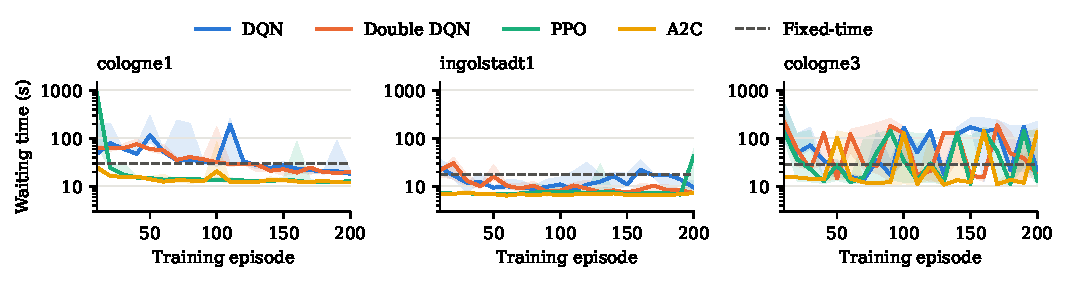
\includegraphics[width=\textwidth]{figures/learning_curves.pdf}
  \caption{Validation waiting time during training.}
  \label{fig:curves}
\end{figure*}

\subsection{Training Stability and Failure Analysis}
Fig.~\ref{fig:curves} shows the complete learning curves, the validation waiting time at every check, on a logarithmic scale so that gridlocked checkpoints remain visible; each line is the median over the five seeds, the band the interquartile range across seeds, and the dashed line fixed-time control. On cologne1 the median A2C and PPO policies beat fixed-time from episodes 10 and 20, and DQN and Double DQN only from 130 and 110; on ingolstadt1 all learners do so within 30 episodes. On cologne3 the validation score oscillates between good and gridlocked policies throughout training: after episode 50, 32\% (A2C), 41\% (PPO, Double DQN) and 48\% (DQN) of the checks are over twice as bad as fixed-time, against 0--11\% on ingolstadt1 and 7--23\% on cologne1.

Failures are rare but severe: a failed episode completes only 31--92\% of trips, against 98.8\% otherwise, which is why mean and median diverge. On cologne3 the median per-seed waiting times of A2C, PPO and Double DQN (13.8, 14.1 and 15.2\,s) are 51--55\% below fixed-time. Selecting the checkpoint on five validation files does not prevent rare failures, since even A2C failed on one of 50 cologne3 test episodes. A likely cause is spillback between adjacent intersections, invisible to the local reward of Section~\ref{sec:problem}.

\subsection{Ablation Study}
\label{sec:ablation}
Table~\ref{tab:ablation} removes one framework component at a time from A2C, the best learner, holding the seeds, hyperparameters, interaction budget and test conditions fixed.

Removing demand-randomized training (C1), i.e.\ training only on the real hour, gives a slightly lower waiting time on that same hour on cologne1 (11.0 vs.\ 11.7\,s), a sign of fitting the training demand; one cologne1 seed then gridlocks at $1.3\times$, and on cologne3 failures rise from 1 to 6 of 50 test episodes (Mann--Whitney $U$ on all test files, $p=0.032$; cologne1 $p=0.42$). Removing policy sharing (C2), i.e.\ one network per cologne3 signal with 34{,}373 instead of 11{,}845 parameters and 3.4 instead of 4.0 CPU-hours of training, gives 4 failures ($p=0.056$). Episodes without gridlock are, however, almost identical in all variants ($1.0\times$: 10.0--10.7\,s), so neither component changes typical performance.

Valid-action masking differs from the full framework only in how the surplus action of the three-phase signal is handled. It also leaves typical performance unchanged and is the most consistent variant on unseen demand (16.8\,$\pm$\,0.7\,s), but it fails in 4 of 50 episodes and in four of five seeds, as often as the ablated variants, and is worse than the unmasked policy over all test files ($p=0.032$). Since a near-identical configuration fails as often as the ablated ones, the low failure count of the full framework is likely due in part to its five seeds, and with five seeds the effect of C1 and C2 on failures is indicative rather than established. Table~\ref{tab:perint} locates the failures: in every variant A2C cuts the mean queue at signals A and B from about 3 vehicles under fixed-time to 0.5--1.7, whereas at signal C, the largest junction, the variants with failing seeds queue almost as much as fixed-time (5.3--6.1 vs.\ 6.8 vehicles).

\begin{table}[t]
\caption{Ablation of A2C (Waiting Time in s)}
\label{tab:ablation}
\centering
\footnotesize
\setlength{\tabcolsep}{2pt}
\resizebox{\columnwidth}{!}{%
\begin{tabular}{|l|l|r|r|r|r|}
\hline
\textbf{Scen.} & \textbf{Variant} & \textbf{Unseen\textsuperscript{a}} & \textbf{Real hour} & \textbf{F} & \textbf{Params} \\
\hline
\multirow{2}{*}{cologne1} & Full (C1 + C2)          & 15.6\,$\pm$\,1.0  & 11.7\,$\pm$\,0.7    & 0 & 11{,}461 \\ \cline{2-6}
                          & $-$C1 (real hour only)  & 25.5\,$\pm$\,25.4 & 11.0\,$\pm$\,0.3    & 1 & 11{,}461 \\
\hline
\multirow{4}{*}{cologne3} & Full (C1 + C2)          & 36.0\,$\pm$\,45.3 & 9.3\,$\pm$\,0.6     & 1 & 11{,}845 \\ \cline{2-6}
                          & $-$C1 (real hour only)  & 66.1\,$\pm$\,66.3 & 122.7\,$\pm$\,227.1 & 6 & 11{,}845 \\ \cline{2-6}
                          & $-$C2 (one per signal)  & 94.6\,$\pm$\,78.4 & 157.1\,$\pm$\,329.8 & 4 & 34{,}373 \\ \cline{2-6}
                          & Full + masking          & 16.8\,$\pm$\,0.7  & 133.6\,$\pm$\,277.1 & 4 & 11{,}845 \\
\hline
\end{tabular}}
\tablenote{Mean $\pm$ s.d.\ over 5 seeds. \textsuperscript{a}The $0.7\times$ and $1.3\times$ test files. F: failed test episodes out of 50. Params: actor and critic.}
\end{table}

\begin{table}[t]
\caption{Mean Queue per Signal on cologne3}
\label{tab:perint}
\centering
\footnotesize
\setlength{\tabcolsep}{4pt}
\begin{tabular}{|l|c|c|c|}
\hline
\textbf{Controller} & \textbf{\makecell{Signal A\\(3 phases)}} & \textbf{\makecell{Signal B\\(4 phases)}} & \textbf{\makecell{Signal C\\(4 phases)}} \\
\hline
Fixed-time          & 3.08 & 3.03 & 6.77 \\
\hline
A2C, shared         & 0.51\,$\pm$\,0.07 & 0.54\,$\pm$\,0.40 & 2.65\,$\pm$\,2.16 \\
\hline
A2C, one per signal & 0.59\,$\pm$\,0.19 & 1.65\,$\pm$\,1.28 & 6.13\,$\pm$\,2.41 \\
\hline
A2C, shared, masked & 0.54\,$\pm$\,0.02 & 0.89\,$\pm$\,0.48 & 5.33\,$\pm$\,2.32 \\
\hline
\end{tabular}
\tablenote{Halted vehicles on each signal's incoming lanes, averaged over the hour and the ten test files; mean $\pm$ s.d.\ over 5 seeds.}
\end{table}

Several challenges remain and set the directions for future work. The most pressing is the rare gridlock of multi-intersection policies, concentrated at the largest junction, which neither validation-based selection, the framework components nor action masking reliably remove; the local, myopic reward is a likely cause, and coordination-aware rewards, a safe fallback to fixed-time control and more training seeds are natural next steps. The test covers demand-level generalization only, the shared policy is tied to the training intersections through its identifier, and the results are simulation-only, so the sim-to-real gap~\cite{rafi2026sim2signal} remains open. Future work will also compress the best learner for roadside devices, building on compact controllers~\cite{xing2022tinylight,gu2024pilight}, and add multi-tier anomaly detection and confidence-aware edge--cloud offloading.
